本节按课堂扩展题的任务一、任务二，完成偶数分频代码审查、最小修复与验证，
以及奇数分频占空比的参数化升级。上板及ILA部分由实验二、三的分工负责，
本节记录软件设计与行为仿真，不重复列入硬件实验内容。

\subsection{任务1：代码找错与原因分析}
\subsubsection{计数范围错误与手推时序}

讲义原偶数分频代码的关键语句为：
\begin{lstlisting}[style=vcode,caption={原代码的计数阈值}]
localparam COUNT = ((DIV_FACTOR) >> 1);
else if(counter == COUNT) begin
    clk_out <= ~clk_out;
    counter <= 0;
end
\end{lstlisting}

当分频系数为10时，\texttt{COUNT=5}。
由于计数从0开始，非阻塞赋值右侧和条件判断均使用该输入边沿到来前的旧值，
原代码依次经历0、1、2、3、4、5六个计数状态才翻转一次输出。
以下从某次计数器清零后推导稳态行为，先排除复位释放边沿带来的额外计数影响。

\begin{table}[H]
\centering
\caption{分频系数为10时，第一次翻转前的手推计数过程}
\begin{tabularx}{\textwidth}{cXX}
\toprule
输入上升沿 & 原代码的动作 & 修复后代码的动作\\
\midrule
第1拍 & 旧值0，更新为1 & 旧值0，更新为1\\
第2拍 & 旧值1，更新为2 & 旧值1，更新为2\\
第3拍 & 旧值2，更新为3 & 旧值2，更新为3\\
第4拍 & 旧值3，更新为4 & 旧值3，更新为4\\
第5拍 & 旧值4，更新为5 & 旧值4，输出翻转并清零\\
第6拍 & 旧值5，输出翻转并清零 & 新半周期开始，更新为1\\
\bottomrule
\end{tabularx}
\end{table}

因此原代码每6拍翻转一次，完整输出周期为12拍，实际为12分频而非10分频：
\[
T_{\mathrm{old}}=2(5+1)T_{\mathrm{in}}=12T_{\mathrm{in}},\qquad
f_{\mathrm{old}}=\frac{f_{\mathrm{in}}}{12}.
\]
一般地，对偶数分频参数$N$，原写法的实际分频比为$N+2$。
原代码的高、低电平都持续6拍，所以稳态占空比仍为50\%；
占空比正确并不能说明分频比也正确。

\begin{figure}[H]
\centering
\setlength{\unitlength}{0.43mm}
\begin{picture}(315,88)
{\color{gray!30}\multiput(65,9)(20,0){13}{\line(0,1){66}}}
\put(0,60){\makebox(60,0)[l]{原代码输出}}
\put(0,28){\makebox(60,0)[l]{修复后输出}}
\put(65,54){\line(1,0){120}}\put(185,54){\line(0,1){12}}
\put(185,66){\line(1,0){120}}\put(305,66){\line(0,-1){12}}
\put(65,22){\line(1,0){100}}\put(165,22){\line(0,1){12}}
\put(165,34){\line(1,0){100}}\put(265,34){\line(0,-1){12}}
\put(265,22){\line(1,0){40}}
\put(65,3){\makebox(0,0){\scriptsize 0}}
\put(85,3){\makebox(0,0){\scriptsize 1}}
\put(105,3){\makebox(0,0){\scriptsize 2}}
\put(125,3){\makebox(0,0){\scriptsize 3}}
\put(145,3){\makebox(0,0){\scriptsize 4}}
\put(165,3){\makebox(0,0){\scriptsize 5}}
\put(185,3){\makebox(0,0){\scriptsize 6}}
\put(205,3){\makebox(0,0){\scriptsize 7}}
\put(225,3){\makebox(0,0){\scriptsize 8}}
\put(245,3){\makebox(0,0){\scriptsize 9}}
\put(265,3){\makebox(0,0){\scriptsize 10}}
\put(285,3){\makebox(0,0){\scriptsize 11}}
\put(305,3){\makebox(0,0){\scriptsize 12}}
\put(65,82){\makebox(240,0){从计数器清零、输出为低开始，每格表示一个输入周期}}
\end{picture}
\caption{手推稳态时序示意：原代码每6拍翻转，修复后每5拍翻转}
\label{fig:ex4_hand_timing}
\end{figure}


\subsubsection{复位极性矛盾及实际效果}

原代码使用\texttt{posedge sys\_rstn}作为复位敏感边沿，
但在内部用\texttt{if(!sys\_rstn)}判断低电平有效复位。
这两者不构成正确的低有效异步复位，其实际仿真行为为：
\begin{enumerate}
    \item 复位从1变0时，下降沿不在敏感表中，模块不会立即清零。
    如果复位低电平持续到下一个输入时钟上升沿，才会由时钟事件触发清零；
    若低脉冲完全落在两个输入上升沿之间，可能被漏掉。
    \item 复位从0变1时，错误的上升沿敏感项会触发该过程。
    此时低有效复位条件不成立，过程反而执行计数或翻转，相当于多执行了一次非时钟触发的状态更新。
\end{enumerate}
因此，不能简单说原代码的复位“完全无效”：它在时钟继续运行且低电平保持足够久时能够清零，
但未实现所需的低有效异步复位，并存在错误的释放边沿行为。
讲义奇数分频模块采用\texttt{negedge sys\_rstn}，与低有效判断一致。

\subsection{任务2：最小修复与仿真对比}
\subsubsection{两处最小修复}

保持原模块端口、16位计数器、单个时序过程及翻转结构，仅修正两处：
\begin{lstlisting}[style=vcode,caption={偶数分频的两处最小修复}]
// 1. Use the falling edge for active-low asynchronous reset.
always @(posedge clk_in or negedge sys_rstn) begin
    if(!sys_rstn) begin
        counter <= 0;
        clk_out <= 0;
    end
    // 2. Count from 0 to COUNT-1: exactly COUNT cycles.
    else if(counter == COUNT - 1) begin
        clk_out <= ~clk_out;
        counter <= 0;
    end
    else begin
        counter <= counter + 1;
    end
end
\end{lstlisting}
修复后从0数到4，共5拍翻转一次，完整周期为10拍，稳态占空比为50\%。

\subsubsection{修复前后的频率与占空比}

扩展测试平台直接提供100MHz输入时钟，将分频参数设为10，
同时驱动原模块与修复模块，以便在同一时间尺度下比较。
这一测试用于隔离分频模块本身，不重复时钟IP的生成与锁定过程。
使用Vivado 2018.2行为仿真，在复位释放后的稳定区间测量两次完整周期，结果如下。

\begin{table}[H]
\centering
\caption{100MHz输入、分频参数为10时的修复前后对比}
\begin{tabular}{lccccc}
\toprule
版本 & 实际分频比 & 周期 & 高电平宽度 & 输出频率 & 占空比\\
\midrule
原代码 & 12 & 120ns & 60ns & 约8.333MHz & 50\%\\
修复后 & 10 & 100ns & 50ns & 10MHz & 50\%\\
\bottomrule
\end{tabular}
\end{table}

图\ref{fig:ex4_frequency}的两组游标分别标出原代码65ns至185ns的完整周期120ns，
以及修复后65ns至165ns的完整周期100ns。
图\ref{fig:ex4_frequency_high}进一步标出原代码65ns至125ns的高电平宽度60ns，
以及修复后65ns至115ns的高电平宽度50ns。
由此得到原代码占空比$60/120=50\%$，修复后占空比$50/100=50\%$，
同时验证了实际分频比与占空比。

\begin{figure}[H]
\centering
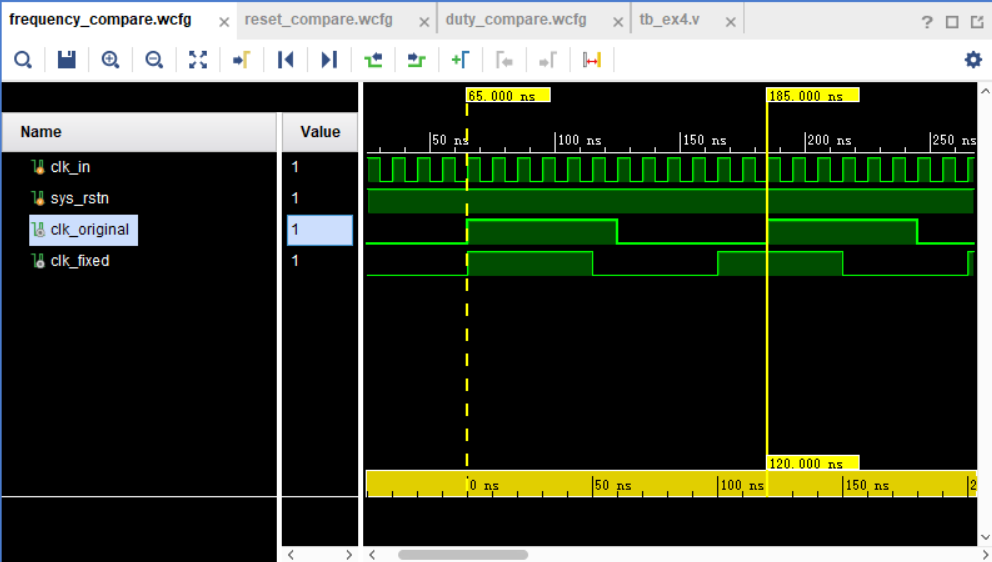
\includegraphics[width=0.90\textwidth]{figures/frequency_original_period.png}\\[0.6em]
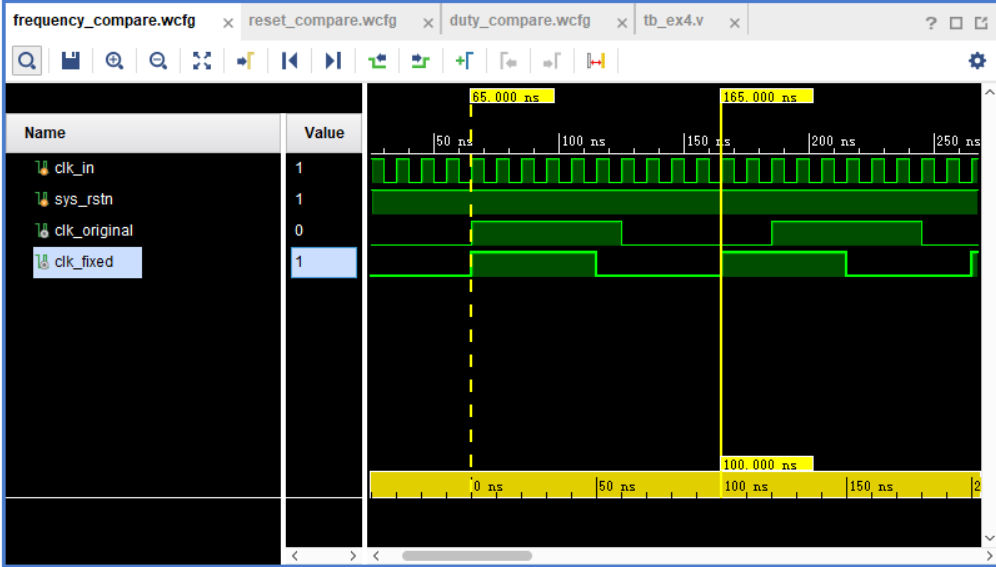
\includegraphics[width=0.90\textwidth]{figures/frequency_fixed_period.png}
\caption{修复前后输出周期的Vivado游标测量：上图原代码120ns，下图修复后100ns}
\label{fig:ex4_frequency}
\end{figure}

\begin{figure}[H]
\centering
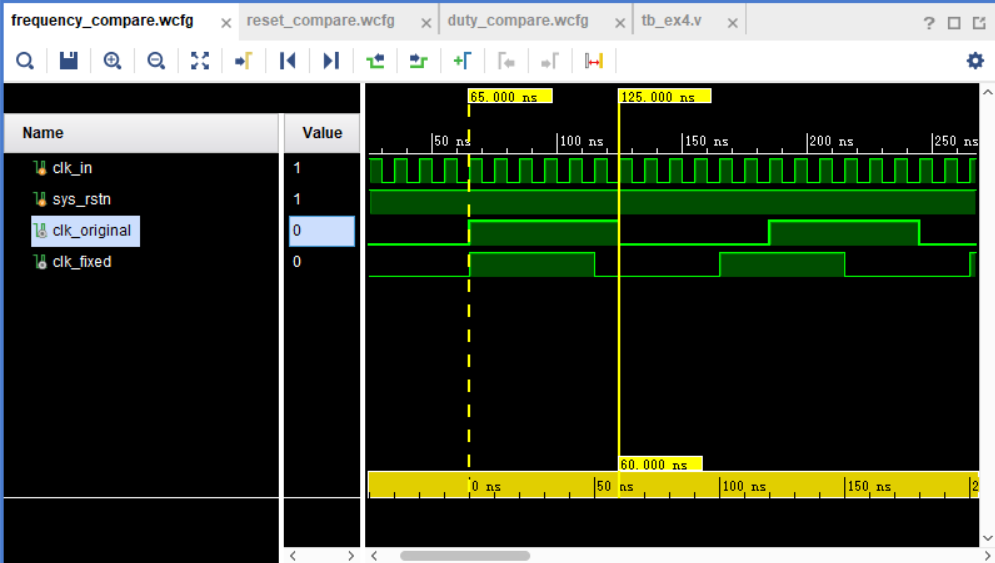
\includegraphics[width=0.90\textwidth]{figures/frequency_original_high.png}\\[0.6em]
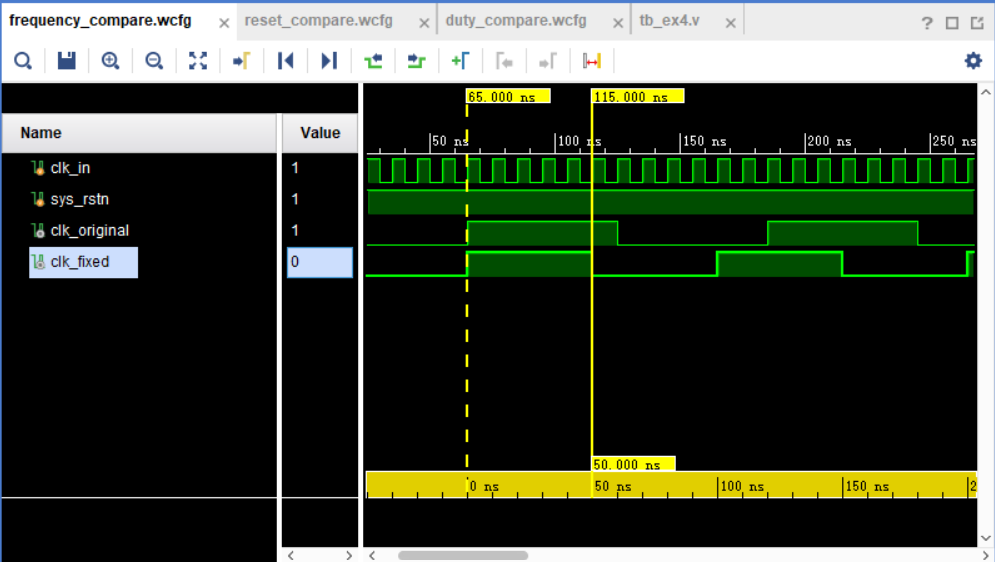
\includegraphics[width=0.90\textwidth]{figures/frequency_fixed_high.png}
\caption{修复前后高电平宽度的Vivado游标测量：上图原代码60ns，下图修复后50ns}
\label{fig:ex4_frequency_high}
\end{figure}


两组输出的高、低电平均等宽，但原代码的周期比目标多2拍。
修复后周期由120ns缩短为100ns，输出频率达到预期10MHz，与手推结果一致。

\subsubsection{复位断言与释放边沿验证}

测试平台在23ns释放初始复位，并在78ns重新拉低测试复位信号。
输入时钟的相邻上升沿为75ns和85ns，因此78ns不与输入上升沿重合。
此时原模块和修复模块的输出原先均为高电平：
\begin{itemize}
    \item 修复模块在78ns立即将输出和计数器清零；
    \item 原模块在78ns仍保持原值，直到85ns的输入上升沿才清零。
\end{itemize}
随后在103ns释放复位，这一时刻同样不与输入上升沿重合。
在104ns检查发现，原模块计数器已因错误的复位上升沿触发而变为1，
修复模块计数器仍为0，直到105ns输入上升沿才开始正常计数。
这些结果由测试平台中的检查语句验证通过。

\begin{figure}[H]
\centering
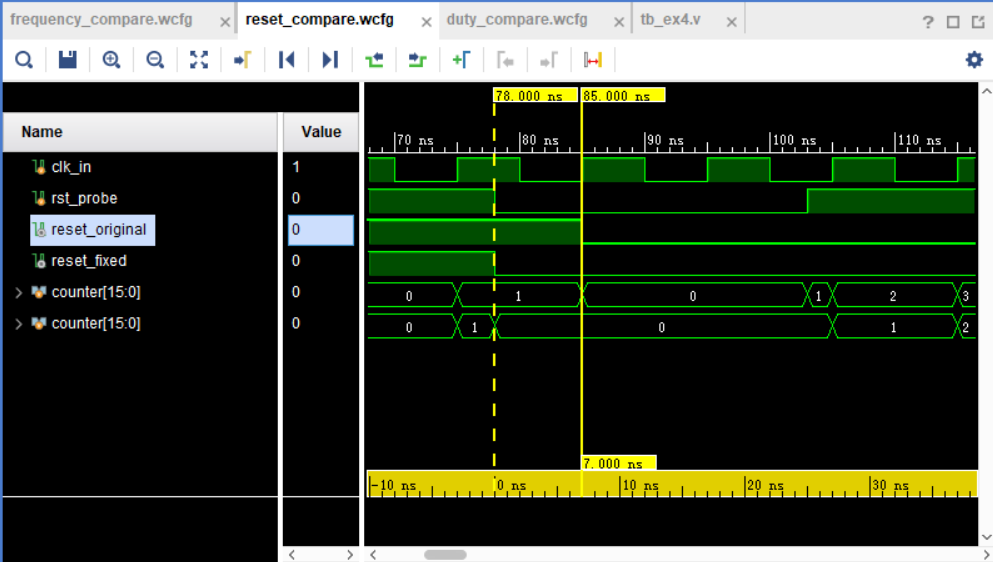
\includegraphics[width=0.90\textwidth]{figures/reset_assertion.png}\\[0.6em]
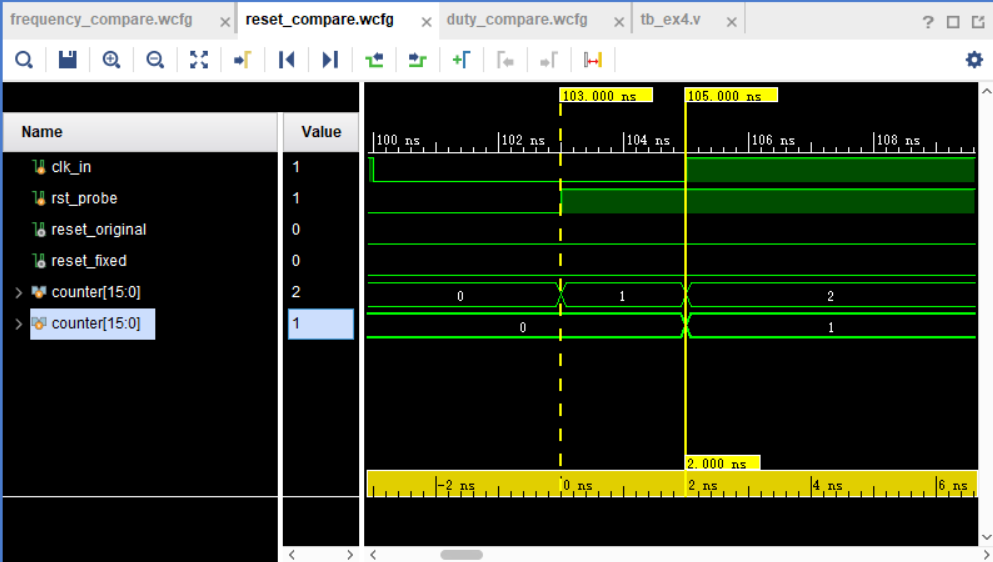
\includegraphics[width=0.90\textwidth]{figures/reset_release.png}
\caption{复位行为的Vivado仿真对比：上图78ns拉低复位，原代码延迟至85ns才清零；下图103ns释放复位，原计数器提前计数，修复后等待105ns输入上升沿}
\label{fig:ex4_reset}
\end{figure}


\subsection{任务2：奇数分频占空比参数化升级}
\subsubsection{参数定义与实现方法}

保留讲义的奇数分频模块，增加带占空比参数的封装模块。
默认占空比为50\%时，直接实例化原有双边沿、双计数器模块，保持原结构和功能；
对于20\%和80\%，用单个上升沿计数器分别安排整拍高、低电平时间。

设奇数分频系数为$N$，目标占空比参数为$P$，整拍模式的高电平拍数为
\[
H=\frac{NP}{100},\qquad
T_{\mathrm{high}}=HT_{\mathrm{in}},\qquad
T_{\mathrm{low}}=(N-H)T_{\mathrm{in}}.
\]
对$N=5$，20\%模式为高1拍、低4拍，80\%模式为高4拍、低1拍。
50\%需要高、低各2.5拍，继续使用原模块的双边沿合成方式。
因此三种配置均为5分频，改变的是占空比而非输出周期。

本实现的参数使用范围为奇数$3\leq N\leq255$、$0<P<100$；
非50\%模式还要求$NP/100$为整数，避免整数除法截断造成目标占空比偏差。
本实验验证$N=5$时的20\%、50\%、80\%三种配置。

\begin{lstlisting}[style=vcode,caption={占空比参数化的奇数分频升级模块}]
`timescale 1ns / 1ps
// DIV_FACTOR为奇数；本实验验证20%、50%、80%。
// 非50%分支要求 DIV_FACTOR*DUTY_CYCLE/100 为整数拍。
module clk_div_odd_duty #(
    parameter DIV_FACTOR = 5,
    parameter DUTY_CYCLE = 50
)(
    input clk_in,
    input sys_rstn,
    output clk_out
);
generate
    if (DUTY_CYCLE == 50) begin : g_duty50
        // 50%模式直接沿用讲义的双边沿、双计数器结构。
        clk_div_odd #(.DIV_FACTOR(DIV_FACTOR)) u_odd (
            .clk_in(clk_in), .sys_rstn(sys_rstn), .clk_out(clk_out)
        );
    end
    else begin : g_integer_duty
        localparam HIGH_COUNT = DIV_FACTOR * DUTY_CYCLE / 100;
        reg [7:0] counter;
        reg clk_reg;
        always @(posedge clk_in or negedge sys_rstn) begin
            if (!sys_rstn) begin
                counter <= 0;
                clk_reg <= 0;
            end
            else begin
                if (counter == DIV_FACTOR - 1)
                    counter <= 0;
                else
                    counter <= counter + 1;
                clk_reg <= (counter < HIGH_COUNT);
            end
        end
        assign clk_out = clk_reg;
    end
endgenerate
endmodule
\end{lstlisting}

\subsubsection{升级模块仿真结果}

三种占空比配置使用同一个100MHz输入时钟和低有效复位，
在稳态区间分别检查完整周期与高电平宽度，结果如下。

\begin{table}[H]
\centering
\caption{100MHz输入、奇数5分频的占空比配置验证}
\begin{tabular}{ccccc}
\toprule
占空比参数 & 周期 & 高电平宽度 & 低电平宽度 & 输出频率\\
\midrule
20\% & 50ns & 10ns & 40ns & 20MHz\\
50\% & 50ns & 25ns & 25ns & 20MHz\\
80\% & 50ns & 40ns & 10ns & 20MHz\\
\bottomrule
\end{tabular}
\end{table}

图\ref{fig:ex4_duty}的两组游标分别位于25ns至35ns、45ns至70ns，
测得20\%模式的高电平宽度为10ns、50\%模式为25ns。
图\ref{fig:ex4_duty80_period}中，80\%模式在25ns至65ns保持高电平，宽度为40ns；
周期测量的游标位于25ns与75ns，这两个时刻同时对应20\%和80\%两路的相邻上升沿，
其周期均为50ns。50\%模式在45ns和95ns的相邻上升沿也相隔50ns。
因此三种模式的占空比分别为$10/50=20\%$、$25/50=50\%$、$40/50=80\%$，
而输出频率均为$1/(50\mathrm{ns})=20\mathrm{MHz}$。

\begin{figure}[H]
\centering
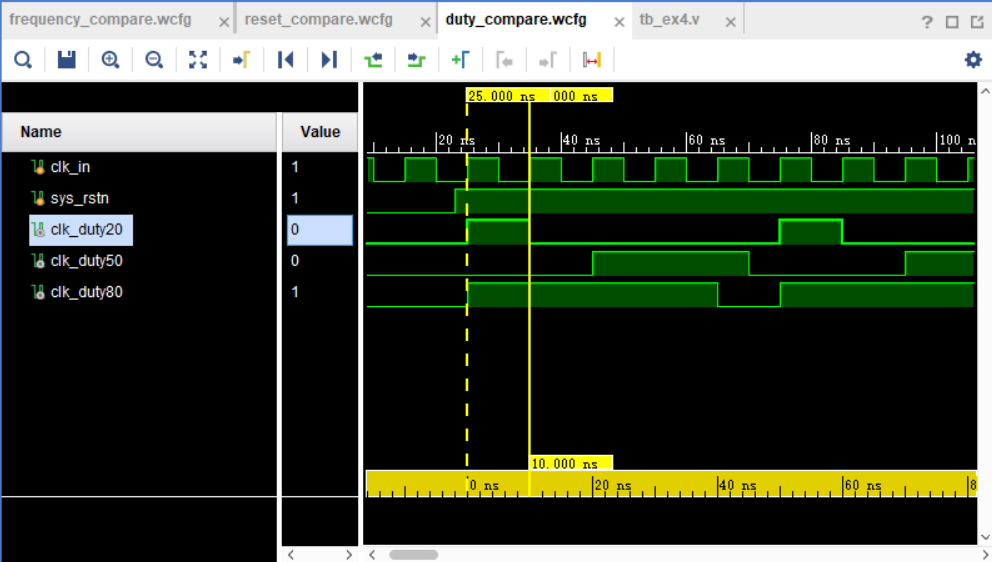
\includegraphics[width=0.90\textwidth]{figures/duty20_high.png}\\[0.6em]
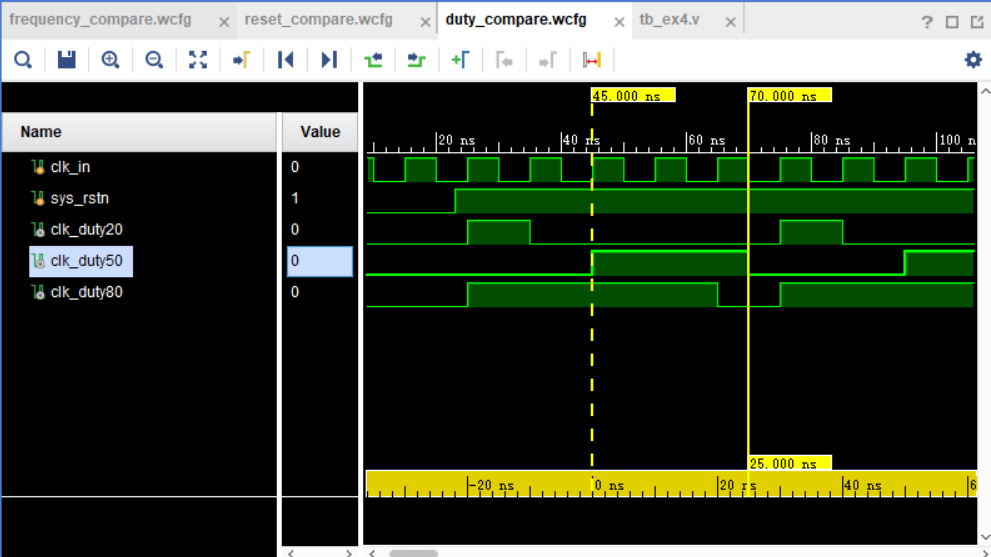
\includegraphics[width=0.90\textwidth]{figures/duty50_high.png}
\caption{占空比参数化模块的高电平宽度测量：上图20\%模式为10ns，下图50\%模式为25ns}
\label{fig:ex4_duty}
\end{figure}

\begin{figure}[H]
\centering
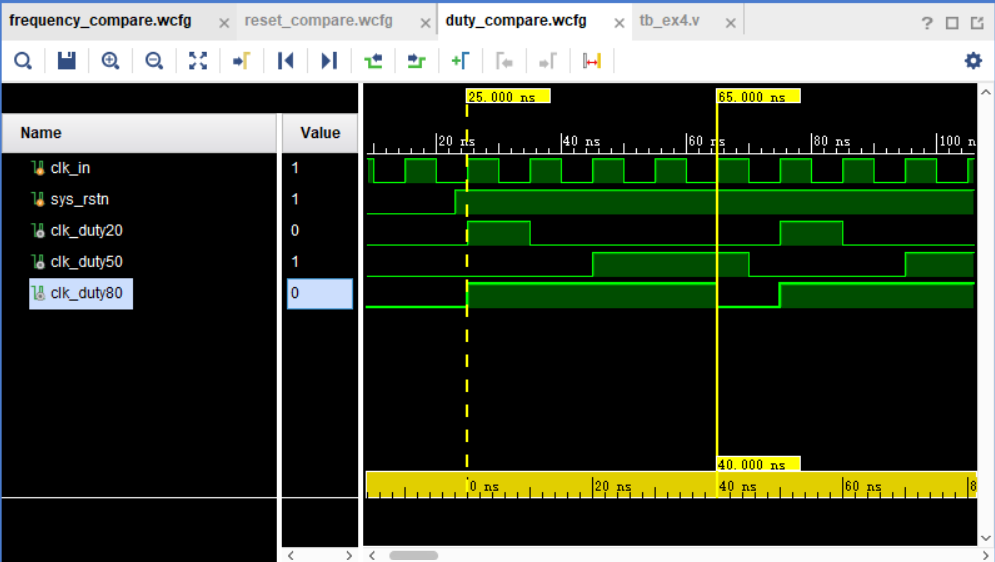
\includegraphics[width=0.90\textwidth]{figures/duty80_high.png}\\[0.6em]
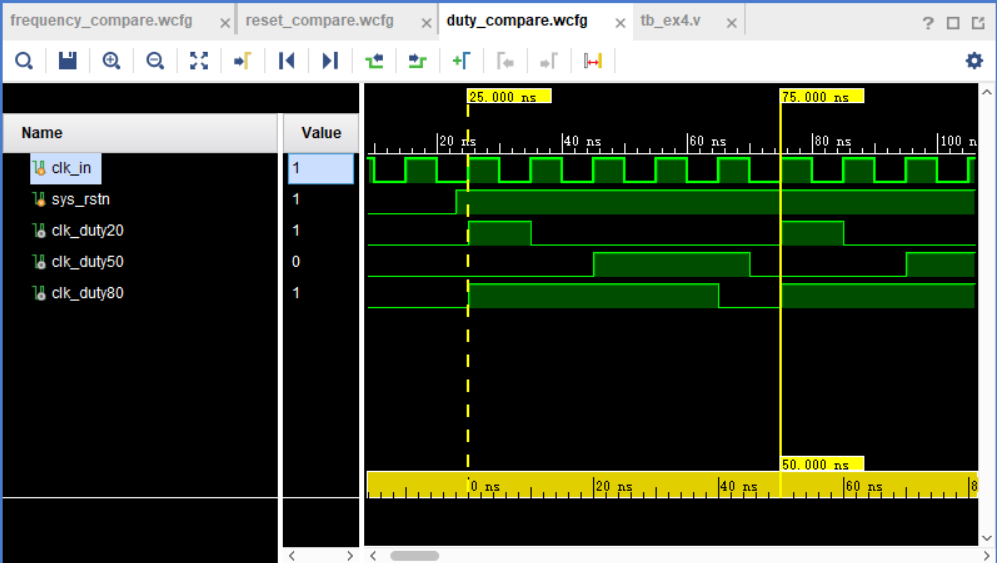
\includegraphics[width=0.90\textwidth]{figures/duty_period.png}
\caption{上图80\%模式高电平宽度为40ns；下图输出周期为50ns，改变占空比后仍保持5分频}
\label{fig:ex4_duty80_period}
\end{figure}


测试平台对上述五组时钟测量（原模块、修复模块及三种占空比）以及复位行为均检查通过。
50\%模式与整拍占空比模式的输出初始相位可以不同，本实验比较其稳态周期及高、低电平宽度。
结果表明，最小修复消除了分频计数误差与复位极性矛盾，
占空比升级在保持5分频的同时实现了20\%、50\%、80\%三种输出。
